\graphicspath{ {imgs/} }
\documentclass[../Thesis.tex]{subfiles}
\begin{document}
\chapter{Classic A/B Testing}

\section{Assumptions and Setup}\label{sec:setup}
This section will take a look at the common approach to A/B Testing as it is also implemented in jabba and other available solutions. To find a common ground for comparison the problem will be abstracted and to a certain degree simplified. This leads to the following definition:

A given test consists of two buckets: Bucket 1 and Bucket 2. Users assigned to Bucket 1 generate actions with a probability $q_1$, for Bucket 2 this probability is $q_2$. The prior distribution for all $q$ is a beta distribution $B(\alpha,\beta)$. This is a convenient choice because it is the conjugate family for the binomial likelihood. 

\begin{figure}[h]
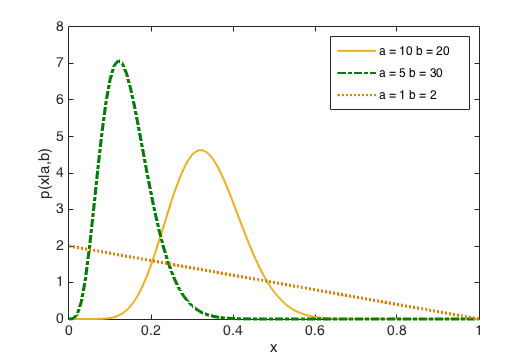
\includegraphics[scale=0.5]{BetaDists.png}
\centering
\title{Different Beta Distributions}
\caption{Different Beta Distributions}
\end{figure}

We also assume no prior knowledge from previous runs when creating the test. This is modeled by the uninformative prior $B(\alpha=1,\beta=1)$. $N_1$ users get assigned to Bucket 1 and $N_2$ to Bucket 2. They generate $k_1$ and $k_2$ actions. The posterior distributions for each individual case is given by:
\begin{align*}
q = f(k|N) &\propto f(N|k)f(k)\\
f_n &= N_n-k_n \\
q_1 = B(k_1+\alpha,f_1+\beta) & = \frac{x^{k_1+\alpha-1}(1-x)^{f_1+\beta -1}}{B(k_1+\alpha,f_1+\beta)} \\
q_2 = B(k_2+\alpha,f_2+\beta) & = \frac{x^{k_2+\alpha-1}(1-x)^{f_2+\beta -1}}{B(k_2+\alpha,f_2+\beta)}
\end{align*}
So each new assignment and each new action will directly alter the distribution parameters. It is important to notice that this model assumes actions to occur directly. The user is assigned to a bucket $n$, produces an action ($k_n + 1$) or not ($f_n + 1$) and leaves again. A user is only measured once -- meaning that the model does not account for actions produced by returning users.
A/B Testing tries to find the posterior probability for $P(q_1>q_2 | k_1,f_1,k_2,f_2)$ the probability that Bucket 1 performs better than Bucket 2 given the collected data. The following section explains three different approaches to that question.

\section{Best Bucket}
The following methods give an overview about strategies that can be implemented to find the best performing bucket among others.

\subsection{Analytic} \label{ssec:analytic}
In general for two random variables $X,Y$ with corresponding probability density functions $f_X,f_Y$ and cumulative density functions $F_X,F_Y$ it holds that: 
\begin{align*}
P(X \geq Y ) &= \iint_{[x>y]} f_X(x)f_Y(y) \,dy\,dx \\
			 &= \iint_{-\infty}^{x} f_X(x)f_Y(y) \,dy\,dx \\
			 &= \int_{-\infty}^{\infty}f_X(x)F_Y(x)\,dx
\end{align*}
In our case with the two given buckets $q_1,q_2$ and the beta distribution that has only non-zero values in the range from 0 to 1 this formula can be simplified to:
\begin{align*}
P(q_1 \geq q_2 ) = \int_{0}^{1}B_{q_1}(k_1,f_1)I_{q_2}(k_2,f_2)\,dx
\end{align*}
Where $I_{q_2}$ is the regularized incomplete beta function. In the paper ``Numerical Computation of Stochastic Inequality Probabilities" the author John D. Cook~\cite{cook2008numerical} uses symmetries of the distribution to arrive at a set of equations that can be used to calculate the problem recursively:
\begin{align*}
g(k_1,f_1,k_2,f_2) &= P(q_1>q_2) \\
h(k_1,f_1,k_2,f_2) &= \frac{B(k_1+k_2,f_1+f_2)}{B(k_1,f_1)B(k_2,f_2)}
\end{align*}
From that Cook shows that starting from a base case all following assignments can be computed by:
\begin{align*}
g(k_1 + 1,f_1,k_2,f_2) &= g(k_1,f_1,k_2,f_2) + h(k_1,f_1,k_2,f_2)/k_1 \\
g(k_1,f_1 + 1,k_2,f_2) &= g(k_1,f_1,k_2,f_2) - h(k_1,f_1,k_2,f_2)/f_1 \\
g(k_1,f_1,k_2 + 1,f_2) &= g(k_1,f_1,k_2,f_2) - h(k_1,f_1,k_2,f_2)/k_2 \\
g(k_1,f_1,k_2,f_2 + 1) &= g(k_1,f_1,k_2,f_2) + h(k_1,f_1,k_2,f_2)/f_2 \\
\end{align*}
This makes sense if the value of $P(q_1>q_2)$ needs to be computed at any time step, since the difference to the previous result can only be an additional action or no-action by a new user. For an arbitrary number $n$ of buckets the formula above resolves to:
\begin{align*}
P(q_1> \max_{i>1}q_i)=\int_{0}^{1}Beta_{q_1}(k_1,f_1) \prod_{i=2}^{n} I_{q_i}(k_i,f_i)\,dx
\end{align*}
In another paper~\cite{cook2006stochastic} Cook and Nadarajah evaluate symmetries for a test with three buckets. The number of applicable symmetries in this case already reduce to:
\begin{align*}
g(k_1,f_1,k_2,f_2,k_3,f_3) &= g(k_1,f_1,k_3,f_3,k_2,f_2) \\
g(k_1,f_1,k_2,f_2,k_3,f_3) &+ g(k_2,f_2,k_3,f_3,k_1,f_1) + g(k_3,f_3,k_1,f_1,k_2,f_2) = 1
\end{align*}
Which corresponds to the fact that $P(q_1>q_2,q_3) = P(q_1>q_3,q_2)$ and that the three possible states of $g$ must sum up to 1. Where the symmetries for $2$ buckets can be used for calculating subsequent states of the test, they can not be generalized for tests with more buckets. 

\subsection{Normal Approximation}\label{ssec:normal_approx}
Different approximations of a normal distribution to the beta distribution can be applied. One detailed derivation is described in ``A normal approximation for beta and gamma tail probabilities'' by Dieter and Hermann~\cite{alfers1984normal}. For larger samples as they are used in the A/B Testing case a simpler approximation can be chosen~\cite{epix}. The following equation should be fulfilled for $B(k,f)$:
\begin{align*}
\frac{k + 1}{k - 1}\approx 0,
\frac{f + 1}{f - 1}\approx 0
\end{align*}
The normal distribution such a beta distribution is given by the following shape:
\begin{align*}
B(k,f)\approx N\left(\frac{k}{k+f},\sqrt{\frac{kf}{(k+f)^2(k+f+1)}} \right)
\end{align*}
The inequality for two normal distributed variables can be solved by:
\begin{align*}
P(X>Y)	&= P(0 > Y - X) \\
			&= P(0 > \mu_Y - \mu_X + (\sigma_X^2 + \sigma_Y^2)^{\frac{1}{2}}Z) \\
			&= P\left(Z < \frac{\mu_X - \mu_Y}{\left(\sigma_X^2 + \sigma_Y^2\right)^{\frac{1}{2}}}\right) \\
			&= \Phi\left(\frac{\mu_X - \mu_Y}{\left(\sigma_X^2 + \sigma_Y^2\right)^{\frac{1}{2}}}\right)
\end{align*}
The gained normal distribution can now be used to perform several hypothesis tests on it. Jabba uses this for example to perform a two tailed hypothesis test to differentiate the performance between buckets while other frameworks use a one tailed testing model. Another important choice in that case is the confidence interval, since it models how reliable the estimate of the action rate is. In jabba the confidence interval is chosen according to ``Interval estimation for a binomial proportion" by Brown et al.~\cite{brown2001interval} the Agresti-Coull interval. The authors find that this interval works well for buckets containing $n \geq 40$ users which is a reasonable assumption, given that those tests are run online and rather deal with several thousand assignments. Other interval estimations may be used leading to more conservative estimates or stricter assumptions.

\subsection{Sampling}
Another method that is more useful for many different buckets is sampling. The following Figure~\ref{fig:SampleBucks} shows a possible situation for a test with many buckets and a high conversion rate for illustrative purposes.
\begin{figure}[h]
\centering
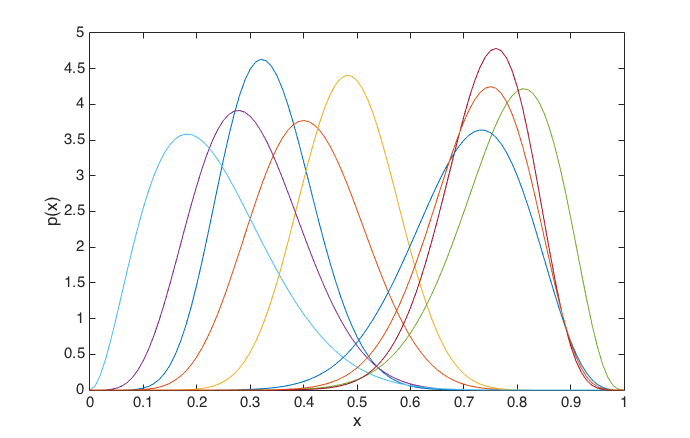
\includegraphics[scale=0.5]{BetaDistributions2.png}
\title{Bucket Distributions}
\caption[Bucket Distributions]{Beta distributions representing the bucket performance during the test}
\label{fig:SampleBucks}
\end{figure}
One algorithm for determining the best bucket among others is algorithm~\ref{alg:BetaSampling}.
\begin{algorithm}
\SetKwData{s}{samples}\SetKwData{num}{num}
\SetKwArray{b}{buckets}\SetKwArray{p}{probabilities}
\SetKwFunction{max}{maxarg}\SetKwFunction{draw}{draw}
\KwIn{\b, \s}
\KwOut{\p}
\BlankLine
\p $\leftarrow$ zeroes \;
\For{ $1$ ... \s }
{
\num $\leftarrow$ \max{\draw{\b}} \;
\p{\num} $\leftarrow$ \p{\num} + $\frac{1}{\s}$ \;
}

\caption[Sampling for best bucket]{Use sampling for determining the best bucket}
\label{alg:BetaSampling}
\end{algorithm}
The accuracy of this method depends on the number of samples that are drawn from each bucket. A simulation in MatLab was conducted to find a reasonable number for the $2$ bucket test. For this random beta distributions have been evaluated using sampling and the basic analytic method described in \ref{ssec:analytic}. For a two-digit exact approximation of the sampling method $20.000$ draws were necessary.


\subsection{Discussion}
The described methods where evaluated for comparing $2$ bucket performances. A generalization to $n$ buckets depends on the chosen method to evaluate the difference between them.

\subsubsection{Analytic}
The analytic approach gives an exact value to the probability that one bucket is performing better than the other, independent of the number of buckets involved in the test. And although the presented symmetries do not generalize to more than two buckets, this method is still superior to the normal approximation in the sense that it is cleaner from the theoretical standpoint, leading to less assumptions about the problem and an easier application.

\subsubsection{Approximation}
When applying the standard techniques of significance testing some general aspects have to be kept in mind. \ref{ssec:normal_approx} already touched on the difference between one- and two-sided hypothesis testing. J. M. Bland et al.~\cite{bland1994statistics} describe in their article ``Statistics Notes: One and two sided tests of significance'' the implication both testing frameworks have on the significance of a result. And though A/B Testing as described here is not tied to clinical trials the underlying issue is the same: when testing one sided the experimenter ignores the possibility that a new feature performs worse than the base implementation. This can lead to the implementation of features that do not really have a significant effect on the customers behavior.
The whole method of significance testing is furthermore again and again source of misconceptions and confusion that also apply to the result of any A/B Test. Goodman describes the common fallacies in his paper ``A dirty dozen: twelve p-value misconceptions'' ~\cite{goodman2008dirty}. The experimenter has therefore to be very careful when interpreting her results.

\subsubsection{Sampling}
Sampling is very easy to implement and depending on the needed precision can be very fast as well. It is more useful if the majority of tests have a lot of different buckets that need to be compared frequently.

\section{Best Assignment}
From the previous section it is clear that the assignment strategy is crucial for a meaningful result of the test. But besides the fact that the assignment should not result in inhomogeneous groups it is not obvious what the overall best strategy is. In the following section several approaches will be described and evaluated against each other.

\subsection{Equal}
For each new user we alternate the assignment equally between the buckets. That means that very bad performing buckets are chosen as often as very well performing ones.

\subsection{Random}
The assignment is based on a draw from a uniform distribution that yields the next bucket. In the long run the assignments are equally distributed as in the for the equal assignment, but can fluctuate in the beginning depending on the concrete draws.

\subsection{Entropy}
Another approach one could think of is distributing the assignments in a way that they minimize the entropy of the inequality across buckets. This makes sense because the desired state at the end of the experiment starting from $P(q_1\geq q_2)=P(q_2\geq q_1)=0.5$ -- a high entropy, should be changed to $P(q_1\geq q_2)\ll P(q_2\geq q_1) \lor P(q_2\geq q_1)\ll P(q_1\geq q_2)$ -- a low entropy. The entropy of $P(q_1\geq q_2)$ is given by:
\begin{align*}
H(q_1,q_2) 	= - P(q_1\geq q_2) \cdot \log_2(P(q_1\geq q_2)) - P(q_2\geq q_1) \cdot \log_2(P(q_2\geq q_1))
\end{align*}
Now it has to be determined which assignment is `better' in the sense of entropy minimization. Consider the following case where a recorded event in a bucket would lead to a huge decrease in the entropy, but it is very unlikely that the user will actually show the behavior. In this case another assignment would still yield the higher information gain. The following factors are used to weight the entropy.
\begin{align*}
w_1 &=\left[\frac{k_1+1}{k_1+f_1+1},\frac{f_1}{k_1+f_1+1}\right] \\
w_2 &=1 - w_1
\end{align*}
The expected entropy with the assignment given to the first bucket, denoted by $q_1^*$, can then be calculated:
\begin{align*}
E(H(q_1^*,q_2)) = w_1\cdot E(q_1^+,q_2) + w_2\cdot E(q_1^-,q_2)
\end{align*}
where $q_1^+$ assumes the user to click and $q_1^-$ not. The formulas for the second bucket can be calculated accordingly. When $E(H(q_1^*,q_2)) < E(H(q_1,q_2^*))$ the next assignment goes to the first bucket. The results of this method can be found in Figure~\ref{fig:AssignmentComp}.

\subsection{Soft Entropy}
But there is a problem with the before described method. When comparing its performance with the random and uniform assignments (see Figure~\ref{fig:AssignmentComp}) it performs worse. This effect appears because the described entropy algorithm optimizes greedily. It starts off with a small offset between the buckets and keeps on focusing on them without trying the other bucket. Different solutions to this situation are possible. The used one in this implementation was adding a softmax algorithm as described in Sutton and Barto's chapter ``Softmax Action Selection''~\cite{sutton1998reinforcement} to the entropy assignment.
\begin{align*}
p(q_1) = \frac{e^{\frac{H(q_1^*,q_2)}{T}}}{e^{\frac{H(q_1^*,q_2)}{T}}+e^{\frac{H(q_1,q_2^*)}{T}}}
\end{align*}
The parameter $T$ called temperature modulates how strong differences between $H(q_1^*,q_2)$ and $H(q_1,q_2^*)$ shall be weighted when calculating the probability that the next assignment goes to Bucket 1 ($p(q_1)$). A high temperature can therefore be used to make the selection of a bucket with higher estimated entropy more likely.
\begin{figure}[ht]
\hfuzz=10cm
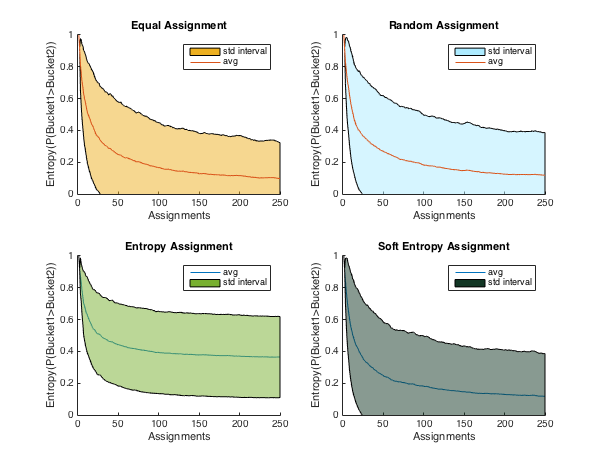
\includegraphics[scale=0.8]{ComparisonAssignments.png}
\centering
\title{Comparison of Assignment Strategies}
\caption{Comparison of Assignment Strategies}
The plots show the performance of the different assignment strategies for randomized buckets. The entropy is used as a measurement of how sure we get over the number of Assignments that one bucket is better/worse than the other.
\label{fig:AssignmentComp}
\end{figure}
\subsection{Discussion}
The used algorithms for the bucket assignment do not differ that much for a two bucket test, see (Figure~\ref{fig:AssignmentComp}). This can be seen in two ways. Either the differences between the presented algorithm do not matter for a test with only two buckets, or equal and random assignment strategies are already very good in what they are doing.
\end{document}